% Official-template-compatible MDPI / Applied Sciences manuscript.
% Replace the body of the official template.tex with this file, or use this file as template.tex.

\documentclass[journal,article,submit,pdftex,moreauthors]{Definitions/mdpi}

\firstpage{1}
\makeatletter
\setcounter{page}{\@firstpage}
\makeatother
\pubvolume{1}
\issuenum{1}
\articlenumber{0}
\pubyear{2026}
\copyrightyear{2026}
%\externaleditor{Firstname Lastname}
\datereceived{}
\daterevised{}
\dateaccepted{}
\datepublished{}

\usepackage{threeparttable}
\usepackage{makecell}
\usepackage{adjustbox}
\usepackage[table]{xcolor}
\usepackage{tikz}
\usepackage{pgfplots}
\usetikzlibrary{arrows.meta,positioning,shapes.geometric,fit,backgrounds}
\pgfplotsset{compat=1.18}

\definecolor{tableheader}{RGB}{228,234,244}
\definecolor{tablerow}{RGB}{247,249,252}
\definecolor{oursrow}{RGB}{236,244,255}
\definecolor{leftband}{RGB}{241,245,250}
\definecolor{accentblue}{RGB}{60,102,168}
\definecolor{accentsoft}{RGB}{232,240,252}
\definecolor{accentgreen}{RGB}{77,144,114}
\definecolor{accentorange}{RGB}{214,140,78}
\newcommand{\TableStyle}{\small\setlength{\tabcolsep}{6pt}\renewcommand{\arraystretch}{1.20}}
\newcommand{\CompactTableStyle}{\footnotesize\setlength{\tabcolsep}{5pt}\renewcommand{\arraystretch}{1.18}}
\newcommand{\SummaryTableStyle}{\small\setlength{\tabcolsep}{7pt}\renewcommand{\arraystretch}{1.24}}

\Title{Exploratory Artificial Intelligence for Automated Social Media Advertising Content Creation and Multi-Objective Creative Optimization}

\newcommand{\orcidauthorA}{0000-0000-0000-000X}
\newcommand{\orcidauthorB}{0000-0000-0000-000X}
\newcommand{\orcidauthorC}{0000-0000-0000-000X}

\Author{Author One $^{1}$\orcidA{}, Author Two $^{1,}$*\orcidB{} and Author Three $^{2}$\orcidC{}}
\AuthorNames{Author One, Author Two and Author Three}

\address{%
$^{1}$ \quad School/Department, University Name, City, Postcode, Country; author1@email.com (A.O.); author2@email.com (A.T.)\\
$^{2}$ \quad School/Department, University Name, City, Postcode, Country; author3@email.com (A.T.)}

\corres{Correspondence: corresponding.author@email.com}

\abstract{Generative artificial intelligence is increasingly used for digital-media advertising, but many practical workflows still rely on one-pass generation followed by manual screening. This improves throughput while offering limited control over creative exploration, limited comparability across alternatives, and weak reproducibility of selection decisions. We propose \textbf{EAI-CO} (Exploratory AI-based Creative Optimization), a framework that treats social-media advertising generation as an exploratory multi-objective optimization problem rather than a one-shot generation task. EAI-CO combines structured brief encoding, controlled candidate exploration, compliance-aware scoring, and iterative refinement. The main benchmark is conducted on a reproducible local \texttt{Qwen2.5-7B-Instruct} backbone over 10 products, 4 audience segments, and 40 product--audience tasks, with comparisons against template, single-pass, open-source, and prompt-engineered baselines, together with four mechanistic ablations. On this benchmark, EAI-CO achieves the highest overall reward (0.805) and significantly outperforms all primary baselines. The ablation results further indicate that diversity preservation, iterative refinement, and audience modeling contribute materially to final performance. A supplementary cross-model validation preserves the same ranking structure on a stronger commercial generator. The findings support a narrower but more defensible conclusion: under a reproducible multi-objective benchmark, exploratory optimization provides stronger automatic creative-evaluation outcomes than one-pass generation alone.}

\keyword{exploratory artificial intelligence; generative AI; digital media; social media advertising; automated content creation; creative optimization}

% Optional for Applied Sciences
%\featuredapplication{An exploratory optimization framework for reproducible, audience-aware social-media advertising content generation.}

\begin{document}

\section{Introduction}

Digital-media advertising has entered a regime in which content scale, audience specificity, and turnaround speed are all expected simultaneously. Social-media campaigns, in particular, require large numbers of tightly formatted creatives that vary by product, segment, and platform context while remaining on-brand, legible, and persuasive. This creates a persistent operational tension: organizations need broad creative coverage, yet the production of high-quality advertising assets remains expensive, iterative, and difficult to standardize.

Generative artificial intelligence is often presented as a solution to this bottleneck because it can produce copy, image prompts, and campaign variants at near-zero marginal generation cost. Recent marketing scholarship has therefore begun to treat generative AI as a meaningful force in marketing strategy, content operations, and creative production \citep{grewal2025,heitmann2024,gastmann2025}. However, a large part of the practical and academic discourse still treats model output as the primary unit of analysis. In many real deployments, the workflow remains narrow: a prompt is written, one or a few candidates are generated, and a human operator informally selects the least problematic result. This approach increases throughput, but it does not solve the core optimization problem of advertising creativity.

Three gaps follow from this limitation. First, the prevailing one-shot workflow provides weak visibility into the creative search process itself. It is therefore difficult to analyze whether quality gains stem from model capability, prompt phrasing, or systematic variation across alternatives. Second, many studies of AI-supported advertising emphasize either generation quality or downstream selection, but do not integrate candidate exploration, candidate comparison, and candidate refinement into one explicit optimization pipeline. Third, reproducible benchmark protocols for creative optimization remain relatively scarce, especially in settings that are feasible under local execution and that expose audience fit, diversity, and compliance as first-class objectives.

These gaps matter because advertising creativity is not a single-output task. In practice, marketers rarely evaluate one isolated creative; they compare alternatives that differ in emotional framing, benefit emphasis, audience targeting, and call-to-action strategy. A useful AI system should therefore do more than produce fluent text. It should search across creative alternatives, preserve strategically meaningful diversity, evaluate candidates under shared objectives, and refine promising directions rather than simply accept the first coherent answer.

This paper addresses that need by proposing \textbf{EAI-CO} (Exploratory AI-based Creative Optimization), a framework that formulates social-media advertising content creation as an exploratory multi-objective optimization problem. EAI-CO integrates structured campaign-brief encoding, exploratory candidate generation, compliance-aware multi-objective evaluation, iterative refinement, and reproducible experiment management. The framework is designed to move AI-assisted advertising from isolated prompt--response interactions toward a controlled search-and-selection process.

The study makes four contributions. First, it formulates automated social-media advertising generation as an exploratory multi-objective optimization problem rather than a one-shot generation task. Second, it proposes EAI-CO, a reproducible framework integrating structured brief encoding, controlled candidate exploration, compliance-aware scoring, and evaluation-guided refinement. Third, it constructs a controlled product--audience benchmark and compares EAI-CO against template, single-pass, open-source, and prompt-engineered baselines under a fixed search budget. Fourth, it provides ablation, audience-wise, runtime, and cross-model analyses to examine mechanism-level contribution and protocol-level transferability.

\section{Related Work}

\subsection{Generative AI as a Marketing and Creative Production Infrastructure}

The first line of relevant work frames generative AI as a broad marketing infrastructure rather than as a narrowly technical text-generation tool. Marketing scholarship has argued that generative AI changes how firms produce, personalize, and adapt customer-facing content, while simultaneously creating new governance and measurement problems \citep{grewal2025,heitmann2024}. Related work in social-media marketing and agency practice further suggests that generative AI affects productivity, task decomposition, and human--AI collaboration rather than only final copy quality \citep{gastmann2025,cui2025}.

This stream is important because it shifts attention from isolated model outputs to organizational workflows. At the same time, much of it remains conceptual, descriptive, or managerial in emphasis. It clarifies why generative AI matters for advertising, but offers less guidance on how to formalize creative generation as a reproducible optimization problem. Our work builds on this stream by operationalizing content production as an explicitly evaluable search process.

\subsection{AI-Generated Advertising Creatives and Commercial Creative Systems}

A second stream focuses more directly on advertising creatives themselves. Recent studies and industrial systems examine creative generation, creative ranking, ad-creative selection, and click-through-rate-oriented optimization. Prior work has shown that creative selection is not a peripheral downstream choice but a component of the advertising decision pipeline itself. Representative examples include joint optimization of ad ranking and creative selection and parallel ranking architectures for ads and creatives in real-time systems \citep{lin2022,yang2024aaai}. In parallel, recent marketing research has shown that generative models can match or even exceed human-created visual marketing content in certain controlled comparisons, especially when evaluated for aesthetic appeal and downstream behavioral response \citep{hartmann2025}.

Despite their relevance, these studies present two limitations for the present problem. First, many are tied to proprietary online systems, industrial logs, or production-serving constraints that are difficult to reproduce in academic settings. Second, they often emphasize either selection quality or output quality, without exposing a transparent candidate-generation and candidate-refinement loop. The present paper contributes a framework-oriented benchmark that preserves practical advertising objectives while remaining tractable under local execution.

\subsection{From Prompt Engineering to Explicit Search and Refinement}

A third stream concerns prompt engineering, iterative generation, and structured refinement. Prompt optimization has become a standard way to improve large-model outputs, including marketing copy and multimodal creative prompts. However, prompt engineering alone often improves results without making the search process itself observable. Even iterative generation methods frequently revise outputs without an explicit account of diversity preservation, elite selection, or controllable mutation across rounds.

This limitation is consequential in advertising because the production task is inherently comparative. Marketers rarely need only one fluent output; they need a set of differentiated options that can be screened for audience fit, compliance, and strategic emphasis. Our approach extends iterative generation by embedding it within a structured search space. Candidates are not merely regenerated; they are explored under defined creative axes and evaluated through a shared reward function. This makes it possible to analyze what is gained by exploration and refinement rather than by prompt fluency alone.

\subsection{Evaluation, Governance, and the Need for Multi-Objective Scoring}

The fourth stream concerns evaluation. Advertising quality is intrinsically multi-objective: a useful creative should be relevant to the product, clear to the viewer, visually plausible, aligned with the target audience, distinct from alternative variants, and compliant with factual or safety constraints. A single scalar criterion such as fluency, lexical diversity, or model confidence is therefore insufficient. More broadly, evaluation scholarship in generated-content research has repeatedly shown that narrow automatic metrics can obscure important quality dimensions and that reproducible evaluation protocols require explicit design choices and reporting discipline \citep{vanderlee2019}.

This issue becomes sharper in digital advertising, where persuasive strength cannot be separated from brand safety, factuality, or audience appropriateness. Our framework therefore adopts a compliance-aware multi-objective perspective. Rather than asking whether a model can produce one persuasive sentence, it asks whether a system can navigate the tradeoff space among relevance, clarity, engagement potential, diversity, and safety in a reproducible way.

\subsection{Positioning of the Present Study}

Taken together, the literature suggests four points. Generative AI is becoming embedded in marketing production systems; creative choice is central to advertising effectiveness; iterative generation is useful but often under-specified; and evaluation must balance multiple objectives rather than rely on a single proxy. What remains underdeveloped is a reproducible framework that combines these elements into one explicit optimization pipeline for social-media advertising. The present study addresses that gap by integrating structured brief encoding, exploratory candidate generation, compliance-aware scoring, iterative refinement, and cross-model validation into a unified benchmarkable system.

\section{Materials and Methods}

\subsection{Methodological Framing}

The objective of the proposed framework is not merely to generate a fluent advertising text, but to model advertising content production as a structured search problem over multiple plausible creative realizations. In this study, the term \emph{exploratory artificial intelligence} refers to a system design in which generation, evaluation, and refinement are explicitly coupled. The methodological premise is that advertising quality emerges from the interaction between candidate diversity, audience conditioning, and objective-guided selection rather than from a single unconditional response from a language model.

Accordingly, EAI-CO is designed as a pipeline with four tightly connected components: (1) structured task encoding, (2) exploratory candidate generation, (3) compliance-aware multi-objective evaluation, and (4) iterative refinement and final selection. This section formalizes the task and describes each component.

\subsection{Task Formulation}

Let a campaign task be denoted as
\begin{equation}
\tau = (p, a, s, c),
\end{equation}
where $p$ denotes a product description, $a$ denotes an audience segment, $s$ denotes a platform or placement context, and $c$ denotes a set of campaign constraints. For a given task $\tau$, the system must generate an advertising creative
\begin{equation}
x = \{\text{headline}, \text{body}, \text{cta}, \text{visual\_prompt}\},
\end{equation}
where the four fields correspond to the minimal textual and multimodal specification used in the benchmark.

The system does not optimize over one isolated output. Instead, it generates a candidate set
\begin{equation}
\mathcal{X}_{\tau} = \{x_1, x_2, \dots, x_n\},
\end{equation}
and seeks to identify
\begin{equation}
x^{*} = \arg\max_{x \in \mathcal{X}_{\tau}} R(x \mid \tau),
\end{equation}
where $R(\cdot)$ is a multi-objective reward defined over both persuasive and governance-related dimensions. This formulation makes the selection logic explicit and allows the framework to be analyzed as an optimization procedure rather than a pure generation interface.

\subsection{Structured Campaign Brief Encoding}

The first stage converts each campaign task into a structured campaign brief. This brief includes product title, product category, selling points, audience segment, platform context, stylistic tone, and explicit constraints. The purpose of this encoding step is methodological rather than cosmetic. It standardizes task specification across all compared methods and reduces variability introduced by inconsistent prompt phrasing.

Formally, the brief encoder maps
\begin{equation}
f_{\mathrm{brief}}: \tau \rightarrow b,
\end{equation}
where $b$ is a normalized structured representation. This representation serves two functions. First, it ensures that all methods receive comparable task information. Second, it enables audience-specific conditioning without requiring ad hoc re-prompting for each baseline. For example, the same product can be paired with different audience segments under the same platform context while preserving a shared core brief.

\subsection{Exploratory Candidate Generation}

The candidate generator does not request one direct response from the underlying model. Instead, it samples from a controlled creative space whose dimensions are defined by a set of exploration axes. In the present benchmark, these axes include emotional style, appeal type, layout style, color direction, CTA style, caption length, and audience pain point.

Each candidate can therefore be expressed as
\begin{equation}
x_i = g(b, z_i),
\end{equation}
where $b$ is the structured brief and $z_i$ is a vector of exploration settings. This design induces meaningful variation across candidates while keeping the search space interpretable. The generator does not aim to maximize randomness; it aims to generate strategically differentiated but still task-relevant variants.

Under the final benchmark configuration, the local and commercial experiments use two rounds of search, two candidates per round, and one elite candidate retained for refinement. This search depth is intentionally moderate. It is large enough to expose the value of exploration but small enough to remain computationally feasible and reproducible under local hardware conditions. The visual-prompt field is retained even though the benchmark does not run a full-scale multimodal image generation study, because visual direction remains part of the creative specification.

\subsection{Compliance-Aware Multi-Objective Evaluation}

Each candidate is evaluated through a shared scoring function that reflects the applied nature of advertising content. The evaluator models quality as a composite of relevance, clarity, aesthetic plausibility, audience fit, predicted engagement, diversity, brand safety, and factuality control. This reflects the assumption that high-performing advertising content is not reducible to fluency or persuasiveness alone.

The local benchmark uses the following weighted reward:
\begin{equation}
R(x) = 0.20r_{\mathrm{rel}} + 0.16r_{\mathrm{clar}} + 0.14r_{\mathrm{aes}} + 0.16r_{\mathrm{aud}} + 0.16r_{\mathrm{eng}} + 0.08r_{\mathrm{div}} + 0.10r_{\mathrm{safe}} - p_{\mathrm{fact}},
\end{equation}
where $r_{\mathrm{rel}}$, $r_{\mathrm{clar}}$, $r_{\mathrm{aes}}$, $r_{\mathrm{aud}}$, $r_{\mathrm{eng}}$, $r_{\mathrm{div}}$, and $r_{\mathrm{safe}}$ represent normalized reward components, and $p_{\mathrm{fact}}$ denotes the factuality penalty term.

The evaluator is intentionally compliance-aware. It does not reward aggressive promotional strength in isolation. Instead, it balances persuasive potential with audience alignment, textual clarity, diversity preservation, and behavioral discipline. This is important because digital advertising systems operate under practical brand and credibility constraints, not under an unconstrained creativity objective.

\subsection{Iterative Refinement and Final Selection}

Once initial candidates are scored, EAI-CO retains the highest-performing elite candidates and refines them through controlled mutation over the exploration axes. The system thus implements a shallow search loop rather than independent repeated prompting. In operational terms, the framework alternates between exploration and exploitation: it first broadens the candidate pool, then refines high-potential regions of the search space.

Let $\mathcal{X}_{\tau}^{(t)}$ denote the candidate set at round $t$. The iterative stage can be summarized as:
\begin{equation}
\mathcal{X}_{\tau}^{(t+1)} = \mathcal{M}\left(\mathcal{E}\left(\mathcal{X}_{\tau}^{(t)}\right)\right),
\end{equation}
where $\mathcal{E}$ denotes elite selection based on the current reward and $\mathcal{M}$ denotes controlled mutation. After the final round, the system returns the candidate with the highest reward. The central methodological point is that refinement is conditioned on prior evaluation rather than performed as unconstrained regeneration.

\subsection{Operational Baselines and Mechanistic Ablations}

The experimental design distinguishes between two comparison layers. The first layer evaluates whether exploratory optimization improves over plausible alternative production workflows. For this purpose, the framework is compared against four primary baselines: \texttt{B0\_Template}, \texttt{B1\_SingleShot\_API}, \texttt{B2\_OpenSource\_Only}, and \texttt{B3\_PromptEngineered\_AI}. These baselines reflect distinct but realistic ways in which automated advertising content may be produced in practice.

The second layer evaluates whether the internal mechanisms of EAI-CO materially contribute to observed performance. For this purpose, four ablations are introduced: \texttt{Ours\_without\_diversity}, \texttt{Ours\_without\_factual\_penalty}, \texttt{Ours\_without\_iterative\_loop}, and \texttt{Ours\_without\_audience\_modeling}. This separation between operational baselines and mechanistic ablations is important for scientific interpretation. The former establishes whether the framework is useful relative to alternative workflows; the latter clarifies why it works.

\subsection{Implementation Logic and Reproducibility Scope}

The implementation is intentionally benchmark-oriented. The search space, reward weights, and method configurations are explicitly fixed in configuration files, and the workflow is executed through script-driven pipelines that produce structured CSV outputs. This design supports reproducibility in three ways. First, it fixes the experimental protocol rather than allowing manual prompt drift. Second, it preserves intermediate and final outputs for downstream analysis. Third, it separates the framework logic from any one backbone model, which makes transfer experiments possible without redefining the method itself.

The scope of reproducibility should nevertheless be stated carefully. The local open-source benchmark is reproducible within the provided code and configuration boundary. The commercial-model experiment is reproducible at the protocol level, but exact token-level outputs may vary across provider-side model revisions and service conditions. This distinction is typical of contemporary AI application studies and is therefore made explicit in the present design.

\section{Experimental Setup}

\subsection{Experimental Objectives}

The experimental design addresses three related questions. First, does the proposed exploratory framework outperform plausible one-pass or rule-based creative production workflows under a fixed product--audience benchmark? Second, do the internal components of the framework, particularly diversity preservation, audience conditioning, factuality control, and iterative refinement, make separable contributions to the observed gain? Third, does the relative advantage of the framework transfer to a stronger commercial backbone under the same task protocol? These questions motivate a two-layer evaluation structure consisting of a reproducible local main benchmark and a fixed-subset commercial cross-model validation.

\subsection{Benchmark Design and Task Construction}

The benchmark is constructed from 10 products crossed with 4 audience segments: students, young professionals, family users, and price-sensitive consumers. This yields 40 product--audience tasks. Each task is instantiated under the same platform-oriented creative brief schema described in the method section, which ensures that all compared methods receive equivalent task information.

For the local main benchmark, 9 final outputs are retained per task: 5 operational comparison methods and 4 mechanistic ablations. This produces 360 evaluated creatives in total. For the commercial validation benchmark, only the 5 primary methods are retained, yielding 200 evaluated creatives. The commercial experiment is intentionally narrower because its function is confirmatory rather than exhaustive.

The benchmark is not intended to approximate the full heterogeneity of real advertising markets. Its purpose is to provide a controlled and repeatable task environment in which differences among generation strategies can be attributed to methodological design rather than uncontrolled prompt drift.

\subsection{Backbone Models and Execution Environment}

\subsubsection{Local Reproducible Backbone}

The main benchmark is executed with a local \texttt{Qwen2.5-7B-Instruct} backbone on an RTX 3090 GPU. This backbone serves as the principal experimental environment because it provides local execution control, fixed configuration management, and stronger reproducibility than a purely provider-hosted workflow.

\subsubsection{Commercial Cross-Model Backbone}

A supplementary transfer experiment is conducted with a stronger commercial API LLM accessed in March 2026. The task set, brief structure, search protocol, evaluator, and analysis logic are kept fixed, while only the generation backbone is replaced. This design makes it possible to interpret the commercial experiment as a protocol-level transfer test rather than as a separate benchmark with altered assumptions.

\subsection{Compared Conditions and Search Budget}

The main experiment compares the full EAI-CO framework against four operational baselines: \texttt{B0\_Template}, \texttt{B1\_SingleShot\_API}, \texttt{B2\_OpenSource\_Only}, and \texttt{B3\_PromptEngineered\_AI}. It additionally evaluates four mechanistic ablations: \texttt{Ours\_without\_diversity}, \texttt{Ours\_without\_factual\_penalty}, \texttt{Ours\_without\_iterative\_loop}, and \texttt{Ours\_without\_audience\_modeling}. This separation mirrors the logic established in the method section: operational baselines test practical usefulness, whereas ablations test causal contribution within the proposed framework.

For both the local benchmark and the commercial transfer benchmark, the search budget is fixed to 2 rounds, 2 candidates per round, and 1 elite candidate retained for refinement. Fixing the search budget is important for interpretability. It ensures that performance differences reflect the structure of exploration and selection rather than unconstrained increases in inference budget.

\subsection{Evaluation Outputs and Statistical Procedure}

All reported metrics are derived from the shared evaluator introduced in the methodological section. The primary reported outcome is the composite reward, which integrates relevance, clarity, aesthetic plausibility, audience fit, predicted engagement, diversity, brand safety, and factuality control. Secondary reported outputs include component-level scores, audience-wise reward summaries, mean latency, and mean model-call counts.

Pairwise comparisons are conducted at the product--audience task level. For each task, the reward of EAI-CO is paired with the reward of each baseline. The analysis reports mean reward differences, paired $t$-test $p$-values, bootstrap 95\% confidence intervals, and Holm--Bonferroni adjusted $p$-values. Audience-fit differences are additionally reported because audience conditioning is central to the problem definition. The commercial transfer experiment follows the same reporting logic, but it is interpreted as protocol-level transfer evidence rather than token-level replication.

\subsection{Reproducibility Boundary and Verification Logic}

The experimental workflow is fully script-driven. Configuration files fix the benchmark composition, method variants, search depth, reward weights, and output destinations. The scripts produce structured CSV outputs for both raw candidate records and aggregated analysis tables. This design reduces researcher degrees of freedom after benchmark construction and makes the execution trace inspectable.

The reproducibility claim should nevertheless be interpreted with appropriate scope. The local \texttt{Qwen2.5-7B-Instruct} benchmark is reproducible within the provided code, configuration, and hardware boundary. The commercial experiment is reproducible at the protocol level, but not necessarily at the exact token-output level, because provider-hosted models may change through backend revisions or service-side nondeterminism. This distinction is made explicit because it affects how evidence from the cross-model experiment should be interpreted.

\subsection{Illustrative Workflow Figures}

Figure~\ref{fig:eai_co_pipeline} summarizes the EAI-CO pipeline from campaign-brief encoding to exploratory candidate generation, multi-objective evaluation, iterative refinement, and final selection. Figure~\ref{fig:candidate_evolution} illustrates candidate evolution under the iterative optimization loop for a representative product--audience task. Figures~\ref{fig:main_reward_bar}--\ref{fig:reward_latency_tradeoff} are designed as result-facing visual summaries and should be placed near the corresponding result subsections in the final layout.

\begin{figure}[H]
\centering
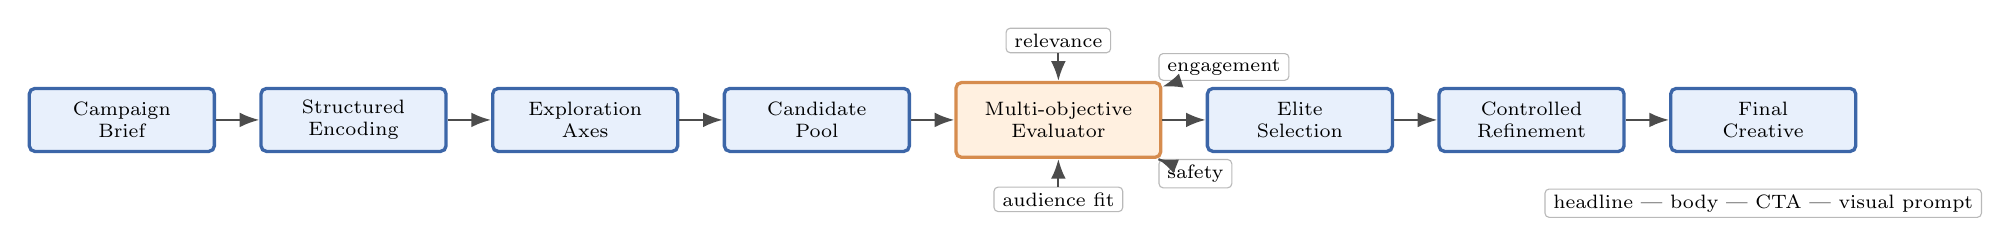
\begin{tikzpicture}[
node distance=0.65cm and 0.55cm,
box/.style={rounded corners=2pt, draw=accentblue, very thick, fill=accentsoft, minimum width=2.35cm, minimum height=0.8cm, align=center, font=\scriptsize},
evalbox/.style={rounded corners=2pt, draw=accentorange, very thick, fill=orange!12, minimum width=2.6cm, minimum height=0.95cm, align=center, font=\scriptsize},
tag/.style={rounded corners=1.5pt, draw=gray!55, fill=white, font=\scriptsize, inner xsep=3pt, inner ysep=2pt},
arrow/.style={-{Latex[length=2.5mm]}, thick, draw=black!70}
]
\node[box] (brief) {Campaign\\Brief};
\node[box, right=of brief] (encode) {Structured\\Encoding};
\node[box, right=of encode] (axes) {Exploration\\Axes};
\node[box, right=of axes] (pool) {Candidate\\Pool};
\node[evalbox, right=of pool] (eval) {Multi-objective\\Evaluator};
\node[box, right=of eval] (elite) {Elite\\Selection};
\node[box, right=of elite] (refine) {Controlled\\Refinement};
\node[box, right=of refine] (final) {Final\\Creative};
\foreach \a/\b in {brief/encode,encode/axes,axes/pool,pool/eval,eval/elite,elite/refine,refine/final}
  \draw[arrow] (\a) -- (\b);
\node[tag, above=0.35cm of eval] (rel) {relevance};
\node[tag, below=0.35cm of eval] (aud) {audience fit};
\node[tag, above right=0.0cm and -0.05cm of eval] (eng) {engagement};
\node[tag, below right=0.0cm and -0.05cm of eval] (safe) {safety};
\draw[arrow, dashed] (rel) -- (eval);
\draw[arrow, dashed] (aud) -- (eval);
\draw[arrow, dashed] (eng) -- (eval);
\draw[arrow, dashed] (safe) -- (eval);
\node[tag, below=0.45cm of final] {headline | body | CTA | visual prompt};
\end{tikzpicture}
\caption{Schematic overview of the EAI-CO framework. The workflow proceeds from campaign-brief encoding to exploratory candidate generation, compliance-aware multi-objective evaluation, elite selection, controlled refinement, and final creative selection.}
\label{fig:eai_co_pipeline}
\end{figure}
\unskip

\begin{figure}[H]
\centering
\begin{tikzpicture}[
node distance=1.35cm and 1.1cm,
step/.style={rounded corners=2pt, draw=accentblue, thick, fill=accentsoft, minimum width=2.3cm, minimum height=0.8cm, align=center, font=\scriptsize},
mini/.style={draw=gray!60, rounded corners=1.5pt, fill=white, minimum width=2.2cm, minimum height=0.5cm, align=left, font=\scriptsize},
arrow/.style={-{Latex[length=2.5mm]}, thick, draw=black!70}
]
\node[step] (gen) {Generate\\Candidates};
\node[step, right=of gen] (score) {Score\\Candidates};
\node[step, right=of score] (elite) {Select\\Elite};
\node[step, right=of elite] (mut) {Mutate\\Axes};
\node[step, right=of mut] (regen) {Regenerate};
\node[step, right=of regen] (final) {Final\\Selection};
\foreach \a/\b in {gen/score,score/elite,elite/mut,mut/regen,regen/final}
  \draw[arrow] (\a) -- (\b);
\draw[arrow, dashed, bend left=28] (regen.north) to node[above, font=\scriptsize] {next round} (score.north);
\node[mini, below=0.85cm of score, anchor=north] (r1a) {R1: emotional appeal\\warm family-oriented copy};
\node[mini, below=0.15cm of r1a.south, anchor=north] (r1b) {R1: price appeal\\discount-oriented copy};
\node[mini, below=0.15cm of r1b.south, anchor=north] (r2) {R2: refined family appeal\\safer, clearer, more audience-specific copy};
\end{tikzpicture}
\caption{Exploration--refinement cycle in EAI-CO. Early-round candidates vary along strategic dimensions, while later-round candidates inherit high-potential directions and are refined under evaluation feedback.}
\label{fig:candidate_evolution}
\end{figure}
\unskip

\begin{table}[H]
\caption{Benchmark configuration and compared methods.}
\label{tab:benchmark_setup}
\centering
\TableStyle
\begin{tabularx}{\textwidth}{>{\columncolor{leftband}}p{3.0cm}X}
\toprule
\rowcolor{tableheader}
Component & Specification \\
\midrule
Main backbone & Local \texttt{Qwen2.5-7B-Instruct} executed on an RTX 3090 GPU \\
Cross-model validation backbone & Stronger commercial API LLM accessed in March 2026 \\
Products & 10 \\
Audience segments & Students, young professionals, family users, and price-sensitive consumers \\
Tasks & 40 product-audience tasks \\
Primary baselines & Template, Single-pass, Open-source, Prompt-Eng., and EAI-CO \\
Ablations & w/o diversity, w/o factuality control, w/o iterative refinement, and w/o audience modeling \\
Search depth & 2 rounds, 2 candidates per round, and 1 elite candidate retained for refinement \\
Reward weights (main benchmark) & relevance 0.20, clarity 0.16, aesthetic 0.14, audience fit 0.16, predicted engagement 0.16, diversity 0.08, and brand safety 0.10 \\
Main evaluated outputs & 360 creatives for the local main experiment; 200 creatives for the commercial cross-model validation \\
\bottomrule
\end{tabularx}
\end{table}


\section{Results}

\subsection{Main Benchmark Results on the Local Backbone}

\begin{figure}[H]
\centering
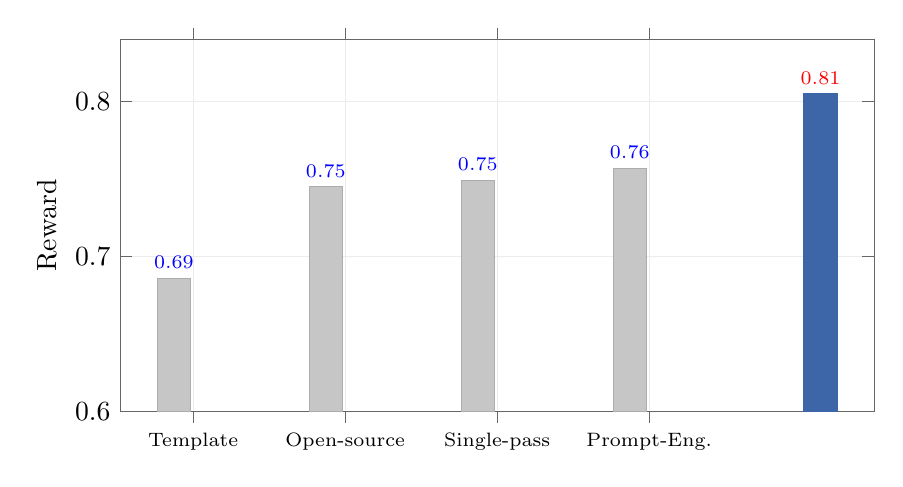
\begin{tikzpicture}
\begin{axis}[
width=0.92\linewidth,
height=6.3cm,
ybar,
bar width=12pt,
ymin=0.60, ymax=0.84,
symbolic x coords={Template,Open-source,Single-pass,Prompt-Eng.,EAI-CO},
xtick=data,
nodes near coords,
nodes near coords align={vertical},
every node near coord/.append style={font=\scriptsize},
xticklabel style={font=\scriptsize, rotate=0, anchor=north},
ylabel={Reward},
axis line style={draw=black!60},
tick style={draw=black!60},
grid=major,
grid style={draw=gray!15},
enlarge x limits=0.12
]
\addplot+[fill=gray!45, draw=gray!65] coordinates {(Template,0.686) (Open-source,0.745) (Single-pass,0.749) (Prompt-Eng.,0.757)};
\addplot+[fill=accentblue, draw=accentblue] coordinates {(EAI-CO,0.805)};
\end{axis}
\end{tikzpicture}
\caption{Main benchmark reward by method on the local \texttt{Qwen2.5-7B-Instruct} backbone. EAI-CO attains the highest reward among the primary methods under the fixed benchmark protocol.}
\label{fig:main_reward_bar}
\end{figure}
\unskip

\begin{table}[H]
\caption{Main benchmark results on the local \texttt{Qwen2.5-7B-Instruct} backbone. Best values among the primary methods are shown in bold.}
\label{tab:qwen_main_results}
\centering
\TableStyle
\rowcolors{2}{tablerow}{white}
\begin{adjustbox}{max width=\textwidth}
\begin{tabular}{lccccc}
\toprule
\rowcolor{tableheader}
Method & Reward & Relevance & Audience Fit & Pred.\ Eng. & Brand Safety \\
\midrule
\rowcolor{oursrow}
EAI-CO & \textbf{0.805} & \textbf{0.912} & \textbf{0.472} & \textbf{0.824} & \textbf{0.995} \\
Prompt-Eng. & 0.757 & 0.792 & 0.439 & 0.785 & 0.940 \\
Single-pass & 0.749 & 0.792 & 0.437 & 0.770 & 0.918 \\
Open-source & 0.745 & 0.805 & 0.431 & 0.765 & 0.934 \\
Template & 0.686 & 0.558 & 0.404 & 0.657 & 1.000 \\
\bottomrule
\end{tabular}
\end{adjustbox}
\end{table}

Table~\ref{tab:qwen_main_results} and Figure~\ref{fig:main_reward_bar} report the main benchmark results obtained on the local \texttt{Qwen2.5-7B-Instruct} backbone. The first result is straightforward: EAI-CO ranks first among all primary methods on the composite reward, achieving \textbf{0.805} relative to 0.757 for Prompt-Eng., 0.749 for Single-pass, 0.745 for Open-source, and 0.686 for Template. The corresponding pairwise comparisons in Table~\ref{tab:significance_cost} indicate that the reward gains over all primary baselines are statistically significant. In practical terms, the full framework improves reward by +0.120 over the template condition ($p = 9.09 \times 10^{-13}$) and remains significantly ahead of the stronger single-pass baselines, with gains of +0.056 over Single-pass ($p = 1.34 \times 10^{-6}$), +0.061 over Open-source ($p = 5.18 \times 10^{-8}$), and +0.048 over Prompt-Eng. ($p = 6.58 \times 10^{-5}$).

The second result is more important for interpretation. The performance advantage is not driven by one inflated component. EAI-CO also attains the strongest audience-fit score (0.4719), the strongest predicted-engagement score (0.8238), and the strongest brand-safety score (0.9945) among the primary methods. This pattern suggests that the framework improves the balance of the creative decision process rather than merely over-optimizing one persuasive dimension at the expense of discipline or audience alignment.

\subsection{Mechanistic Evidence from the Ablation Study}

\begin{figure}[H]
\centering
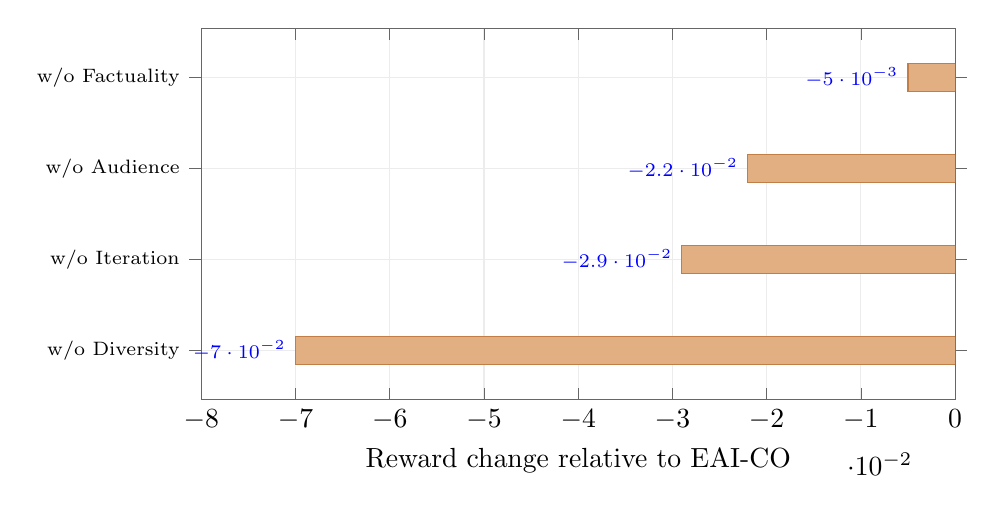
\begin{tikzpicture}
\begin{axis}[
width=0.92\linewidth,
height=6.3cm,
xbar,
xmin=-0.08, xmax=0.0,
symbolic y coords={w/o Diversity,w/o Iteration,w/o Audience,w/o Factuality},
ytick=data,
nodes near coords,
nodes near coords align={horizontal},
every node near coord/.append style={font=\scriptsize},
yticklabel style={font=\scriptsize},
xlabel={Reward change relative to EAI-CO},
axis line style={draw=black!60},
tick style={draw=black!60},
grid=major,
grid style={draw=gray!15},
enlarge y limits=0.18
]
\addplot+[fill=accentorange!70, draw=accentorange!90!black] coordinates {(-0.070,w/o Diversity) (-0.029,w/o Iteration) (-0.022,w/o Audience) (-0.005,w/o Factuality)};
\end{axis}
\end{tikzpicture}
\caption{Ablation waterfall-style summary of reward degradation relative to the full EAI-CO framework. Diversity removal causes the largest decline, followed by iterative refinement and audience modeling.}
\label{fig:ablation_waterfall}
\end{figure}
\unskip

\begin{table}[H]
\caption{Ablation results on the local \texttt{Qwen2.5-7B-Instruct} benchmark. Negative reward gaps indicate degradation relative to the full EAI-CO framework.}
\label{tab:qwen_ablation}
\centering
\TableStyle
\rowcolors{2}{tablerow}{white}
\begin{adjustbox}{max width=\textwidth}
\begin{tabular}{lcccccc}
\toprule
\rowcolor{tableheader}
Method & Reward & Reward Gap vs. Ours & Audience Fit & Audience-Fit Gap & Pred.\ Eng. & Brand Safety \\
\midrule
\rowcolor{oursrow}
EAI-CO & \textbf{0.805} & 0.000 & \textbf{0.472} & 0.000 & \textbf{0.824} & 0.995 \\
w/o Factuality & 0.801 & -0.005 & 0.469 & -0.003 & 0.819 & 0.813 \\
w/o Audience & 0.783 & -0.022 & 0.396 & -0.076 & 0.810 & \textbf{1.000} \\
w/o Iteration & 0.776 & -0.029 & 0.442 & -0.030 & 0.796 & 0.967 \\
w/o Diversity & 0.735 & -0.070 & 0.456 & -0.016 & 0.815 & 0.989 \\
\bottomrule
\end{tabular}
\end{adjustbox}
\end{table}

Table~\ref{tab:qwen_ablation} and Figure~\ref{fig:ablation_waterfall} clarify where the gain comes from. The full method remains superior to all ablated variants, which is necessary for claiming that the contribution lies in the full optimization design rather than in a single isolated heuristic. The largest degradation occurs when diversity preservation is removed (-0.0702), indicating that breadth of exploration is not peripheral but central to final creative quality. Removing the iterative loop reduces reward by -0.0291, showing that evaluation-conditioned refinement adds value beyond first-pass candidate generation. Removing audience modeling lowers reward by -0.0218 and reduces audience fit from 0.4719 to 0.3960, which provides direct evidence that persona-aware conditioning is functionally active in the optimization trajectory.

The factual-penalty ablation is closer to the full model (-0.0045) than the other ablations. That result should not be read as evidence that compliance-aware controls are irrelevant. The more defensible interpretation is narrower: factual safeguards can be integrated into the optimization loop with only a limited cost in persuasive reward, while still improving the procedural discipline of the system. For an applied advertising setting, this is a meaningful result because practical content systems are judged partly by their ability to stay within credibility and governance constraints.

\subsection{Audience-Wise Robustness}

\begin{table}[H]
\caption{Audience-wise reward on the local \texttt{Qwen2.5-7B-Instruct} benchmark. Best values within each audience segment are shown in bold.}
\label{tab:qwen_audience}
\centering
\SummaryTableStyle
\rowcolors{2}{tablerow}{white}
\begin{adjustbox}{max width=\textwidth}
\begin{tabular}{lcccc}
\toprule
\rowcolor{tableheader}
Method & Students & Young Professionals & Family Users & Price-sensitive Consumers \\
\midrule
\rowcolor{oursrow}
EAI-CO & \textbf{0.810} & \textbf{0.805} & \textbf{0.815} & \textbf{0.791} \\
Prompt-Eng. & 0.717 & 0.755 & 0.779 & 0.776 \\
Single-pass & 0.765 & 0.736 & 0.739 & 0.758 \\
Open-source & 0.723 & 0.739 & 0.766 & 0.750 \\
Template & 0.680 & 0.688 & 0.699 & 0.676 \\
\bottomrule
\end{tabular}
\end{adjustbox}
\end{table}

Table~\ref{tab:qwen_audience} examines whether the overall effect is concentrated in one favorable audience subgroup. It is not. EAI-CO ranks first for family users (0.8147), students (0.8098), young professionals (0.8050), and price-sensitive consumers (0.7908). This consistency matters because the core claim of the paper is audience-conditioned optimization rather than generic copy improvement. A framework that only improved aggregate reward while failing to generalize across audience segments would offer weaker evidence for that claim. The present results instead indicate that the relative gain persists across materially different audience logics.

\subsection{Runtime Characteristics}

\begin{table}[H]
\caption{Efficiency and compliance profile on the local \texttt{Qwen2.5-7B-Instruct} benchmark. Calls denote the average number of model invocations required to produce the complete creative package.}
\label{tab:qwen_efficiency_profile}
\centering
\SummaryTableStyle
\rowcolors{2}{tablerow}{white}
\begin{adjustbox}{max width=0.86\textwidth}
\begin{tabular}{lcccc}
\toprule
\rowcolor{tableheader}
Method & Diversity & Factual Penalty & Calls & Latency (ms) \\
\midrule
\rowcolor{oursrow}
EAI-CO & 0.769 & 0.001 & 8.0 & 11114 \\
Prompt-Eng. & 0.860 & 0.011 & 4.0 & 2727 \\
Single-pass & \textbf{0.866} & 0.013 & 4.0 & 2780 \\
Open-source & 0.863 & 0.012 & 3.0 & 2707 \\
Template & \textbf{1.000} & 0.000 & 0.0 & 1 \\
\bottomrule
\end{tabular}
\end{adjustbox}
\end{table}

\begin{figure}[H]
\centering
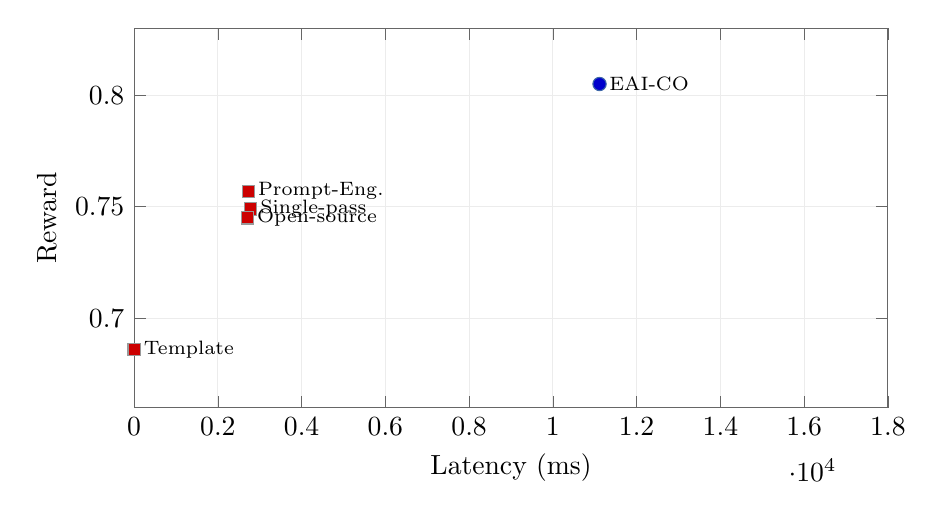
\begin{tikzpicture}
\begin{axis}[
width=0.92\linewidth,
height=6.4cm,
xlabel={Latency (ms)},
ylabel={Reward},
xmin=0, xmax=18000,
ymin=0.66, ymax=0.83,
grid=major,
grid style={draw=gray!15},
axis line style={draw=black!60},
tick style={draw=black!60}
]
\addplot+[only marks, mark=*, mark size=2.4pt, accentblue] coordinates {(11114,0.805)};
\addplot+[only marks, mark=square*, mark size=2.2pt, gray!80] coordinates {(2727,0.757) (2780,0.749) (2707,0.745) (1,0.686)};
\node[font=\scriptsize, anchor=west] at (axis cs:11114,0.805) {EAI-CO};
\node[font=\scriptsize, anchor=west] at (axis cs:2727,0.757) {Prompt-Eng.};
\node[font=\scriptsize, anchor=west] at (axis cs:2780,0.749) {Single-pass};
\node[font=\scriptsize, anchor=west] at (axis cs:2707,0.745) {Open-source};
\node[font=\scriptsize, anchor=west] at (axis cs:1,0.686) {Template};
\end{axis}
\end{tikzpicture}
\caption{Reward--latency trade-off across the primary methods on the local benchmark. EAI-CO occupies the expected high-cost, high-reward region of the design space.}
\label{fig:reward_latency_tradeoff}
\end{figure}
\unskip

\begin{table}[H]
\caption{Statistical comparison of EAI-CO against primary baselines. Pairwise comparisons are conducted at the product--audience task level using paired tests, bootstrap confidence intervals, and Holm--Bonferroni correction.}
\label{tab:significance_cost}
\centering
\SummaryTableStyle
\rowcolors{2}{tablerow}{white}
\begin{tabularx}{\textwidth}{lccccc}
\toprule
\rowcolor{tableheader}
Baseline & $\Delta$ Reward & 95\% CI & $p$-value & Adjusted $p$ & $\Delta$ Audience Fit \\
\midrule
Template & +0.120 & [0.109, 0.130] & $3.72\times10^{-23}$ & $1.49\times10^{-22}$ & +0.068 \\
Single-pass & +0.056 & [0.035, 0.076] & $5.11\times10^{-6}$ & $1.02\times10^{-5}$ & +0.035 \\
Open-source & +0.061 & [0.043, 0.078] & $9.47\times10^{-8}$ & $2.84\times10^{-7}$ & +0.041 \\
Prompt-Eng. & +0.048 & [0.027, 0.069] & $6.71\times10^{-5}$ & $6.71\times10^{-5}$ & +0.033 \\
\bottomrule
\end{tabularx}
\end{table}

Table~\ref{tab:qwen_efficiency_profile}, Table~\ref{tab:significance_cost}, and Figure~\ref{fig:reward_latency_tradeoff} report the computational cost of this gain. EAI-CO requires 8.0 mean model calls per task and 11114 ms mean latency, whereas the single-pass baselines require approximately 3--4 model calls and 2700--2800 ms mean latency. The increase is substantial but unsurprising, because the proposed method explicitly exchanges additional inference budget for structured exploration and selective refinement. The relevant question is therefore not whether the framework is cheaper than one-shot generation; it is whether the additional cost is commensurate with the observed gain. For the intended offline campaign-design scenario, the answer is affirmative.

\subsection{Cross-Model Validation on a Commercial API LLM}

\begin{table}[H]
\caption{Cross-model validation results on a stronger commercial API LLM accessed in March 2026. Best values among the primary methods are shown in bold.}
\label{tab:gpt_cross_model}
\centering
\CompactTableStyle
\rowcolors{2}{tablerow}{white}
\begin{adjustbox}{max width=\textwidth}
\begin{tabular}{lccccccccc}
\toprule
\rowcolor{tableheader}
Method & Reward & Relevance & Clarity & Audience Fit & Diversity & Pred.\ Eng. & Brand Safety & Penalty & Latency (ms) \\
\midrule
\rowcolor{oursrow}
EAI-CO & \textbf{0.996} & \textbf{1.000} & \textbf{0.739} & \textbf{0.756} & 0.804 & \textbf{0.851} & \textbf{1.000} & 0.000 & 17129 \\
Open-source & 0.975 & 0.987 & 0.737 & 0.645 & 0.863 & 0.815 & \textbf{1.000} & 0.000 & 6444 \\
Single-pass & 0.974 & 0.987 & 0.694 & 0.718 & \textbf{0.866} & 0.821 & 0.989 & 0.011 & 6188 \\
Prompt-Eng. & 0.973 & 0.984 & 0.693 & 0.699 & 0.860 & 0.828 & 0.989 & 0.012 & 10776 \\
Template & 0.840 & 0.558 & 0.920 & 0.404 & 1.000 & 0.657 & \textbf{1.000} & 0.000 & 1 \\
\bottomrule
\end{tabular}
\end{adjustbox}
\end{table}

Table~\ref{tab:gpt_cross_model} evaluates whether the main finding is specific to the local open-source backbone. The answer is again negative. Under a stronger commercial API LLM, the same ranking structure is preserved, with EAI-CO remaining first at \textbf{0.996}, followed by Open-source (0.975), Single-pass (0.974), Prompt-Eng. (0.973), and Template (0.840). The gains relative to all primary baselines remain statistically significant, including +0.156 over Template ($p = 1.54 \times 10^{-8}$), +0.022 over Single-pass ($p = 1.41 \times 10^{-3}$), +0.021 over Open-source ($p = 6.42 \times 10^{-4}$), and +0.023 over Prompt-Eng. ($p = 1.01 \times 10^{-3}$).

The audience-wise ordering is likewise preserved, with EAI-CO ranking first for family users (0.9950), price-sensitive consumers (0.9938), students (1.0000), and young professionals (0.9939). The effect sizes are compressed because the commercial backbone operates closer to the ceiling of the current evaluator, but the preservation of rank order remains informative. It reduces the risk that the main result is an artifact of a single local backbone and supports a protocol-level transfer interpretation.

\section{Discussion}

\subsection{The Primary Gain Comes from Optimization Structure}

Taken together, the results support a clear interpretation: the main gain arises from optimization structure rather than from any one generator in isolation. Across both the local benchmark and the commercial transfer benchmark, the proposed framework remains superior to one-pass generation and template-based workflows. This suggests that, for social-media advertising, content quality should be modeled as a search, evaluation, and selection problem rather than as a direct-response text generation task.

\subsection{Diversity and Iteration Are Material Design Factors}

The ablation results further sharpen that interpretation. Diversity preservation and iterative refinement emerge as the main structural sources of improvement. This matters conceptually as well as empirically. It indicates that the framework does not benefit merely from generating more text; it benefits from preserving strategically differentiated directions long enough for the evaluator to discriminate among them and from refining high-potential candidates instead of restarting generation from scratch. In that sense, the method operationalizes a recognizable creative workflow while still keeping it measurable and reproducible.

\subsection{Audience Modeling Has Functional Value}

The audience-modeling ablation shows that personalization is not functioning here as a superficial rhetorical wrapper. Once persona conditioning is removed, both reward and audience fit decline. That pattern implies that audience information is shaping candidate ranking and refinement, not merely decorating otherwise generic copy. For a digital-media application context, this point is important because the theoretical value of automated creative systems depends partly on whether they can adapt content structure to audience logic rather than simply scale generic message production.

\subsection{Compliance-Aware Scoring Is Practically Necessary}

The factuality-control result should be read in applied rather than purely mathematical terms. The relatively small reward gap between the full framework and the no-penalty ablation indicates that compliance-aware controls can be incorporated without collapsing persuasive performance. This is operationally significant. In realistic advertising settings, a system that produces marginally more aggressive copy at the cost of weaker credibility or governance discipline is not necessarily preferable. The present findings therefore support the inclusion of compliance-aware scoring as part of the method design even when its incremental reward contribution is smaller than that of diversity or iteration.

\subsection{Cross-Model Transfer Strengthens the Contribution}

The commercial-model experiment should be interpreted narrowly but usefully. It is not the primary source of effect-size evidence, because the stronger backbone compresses scores toward the upper bound of the evaluator. Its value lies elsewhere: it shows that the relative advantage of EAI-CO survives a backbone substitution while the task protocol remains fixed. This materially strengthens the paper, because it shifts the contribution away from backbone-specific behavior and toward the framework-level logic of exploratory generation, multi-objective evaluation, and refinement.

\subsection{Limitations}

The present study also has clear limits. First, it does not evaluate real platform click-through or conversion outcomes, so the claims should remain restricted to automatic reward superiority, predicted engagement, audience-conditioned quality, and cross-model ranking consistency. Second, the current submission does not include a completed human-evaluation study. That omission does not negate the reported automatic and transfer results, but it does constrain the strength of any claim about end-user preference. Third, the benchmark is methodologically useful yet still smaller and more controlled than a production-scale industrial evaluation environment. Future work should therefore expand benchmark diversity, strengthen multimodal realization, and connect exploratory optimization more directly to downstream deployment outcomes.

\section{Conclusions}

This paper presented EAI-CO, a framework that treats social-media advertising content creation as an exploratory multi-objective optimization problem rather than a one-pass text-generation task. On a reproducible local benchmark built on \texttt{Qwen2.5-7B-Instruct}, the framework significantly outperformed template-based and single-pass baselines, and the ablation results showed that diversity preservation, iterative refinement, and audience modeling each contribute materially to the observed gain. The fixed-subset experiment on a stronger commercial API LLM further preserved the same method ranking, supporting a transfer interpretation at the protocol level.

The substantive implication is that AI-assisted advertising systems should not be evaluated solely by the fluency of individual outputs or by backbone strength alone. A more defensible scientific direction is to model creative production as a controlled process of exploration, evaluation, and refinement under explicit audience, quality, and compliance constraints. Within the limits of automatic and transfer-based evaluation, the present study provides evidence that such a framing yields more reliable creative optimization than one-pass generation alone and offers a stronger methodological foundation for future research in digital-media content automation.

\authorcontributions{Conceptualization, A.O. and A.T.; methodology, A.O. and A.T.; software, A.O.; validation, A.O. and A.T.; formal analysis, A.O.; investigation, A.O.; resources, A.T.; data curation, A.O.; writing---original draft preparation, A.O.; writing---review and editing, A.O., A.T. and A.T.; visualization, A.O.; supervision, A.T.; project administration, A.T. All authors have read and agreed to the published version of the manuscript.}

\funding{This research received no external funding.}

\institutionalreview{Not applicable.}

\informedconsent{Not applicable.}

\dataavailability{The code, configuration files, and structured benchmark summaries supporting the reported results are available in the public project repository: \url{https://github.com/zhangdh2019-sudo/paper-digital-media}. Large generated outputs are omitted from version control for repository hygiene but can be made available by the corresponding author upon reasonable request.}

\acknowledgments{The authors acknowledge the use of local GPU resources for the reproducible open-source benchmark and API-based access for the commercial-model transfer experiment.}

\conflictsofinterest{The authors declare no conflicts of interest.}

\abbreviations{Abbreviations}{
\noindent
\begin{tabular}{@{}ll}
AI & Artificial intelligence\\
CTA & Call to action\\
EAI-CO & Exploratory AI-based Creative Optimization\\
CTR & Click-through rate
\end{tabular}
}

\begin{adjustwidth}{-\extralength}{0cm}
\reftitle{References}
\begin{thebibliography}{999}

\bibitem[Grewal et~al.(2025)]{grewal2025}
Grewal, D.; Satornino, C.B.; Davenport, T.; Guha, A.
How Generative AI Is Shaping the Future of Marketing.
\emph{J. Acad. Mark. Sci.} \textbf{2025}, \emph{53}, 1220--1242.

\bibitem[Heitmann(2024)]{heitmann2024}
Heitmann, M.
Generative AI for Marketing Content Creation: New Rules for an Old Game.
\emph{NIM Mark. Intell. Rev.} \textbf{2024}, \emph{16}, 10--17.

\bibitem[Gastmann(2025)]{gastmann2025}
Gastmann, J.
Strategising with Generative AI: Productivity Gains in Social Media Marketing.
\emph{J. Mark. Commun.} \textbf{2025}, published online ahead of print.

\bibitem[Cui et~al.(2025)]{cui2025}
Cui, W.; Liu, M.J.; Yuan, R.
Exploring the Integration of Generative AI in Advertising Agencies: A Co-Creative Process Model for Human--AI Collaboration.
\emph{J. Advert. Res.} \textbf{2025}, 1--23.

\bibitem[Lin et~al.(2022)]{lin2022}
Lin, K.; Zhang, X.; Li, F.; Wang, P.; Long, Q.; Deng, H.; Xu, J.; Zheng, B.
Joint Optimization of Ad Ranking and Creative Selection.
In \emph{Proceedings of the 45th International ACM SIGIR Conference on Research and Development in Information Retrieval}; ACM: New York, NY, USA, 2022; pp. 2627--2631.

\bibitem[Yang et~al.(2024a)]{yang2024aaai}
Yang, Z.; Sang, L.; Wang, H.; Chen, W.; Wang, L.; He, J.; Peng, C.; Lin, Z.; Gan, C.; Shao, J.
Parallel Ranking of Ads and Creatives in Real-Time Advertising Systems.
In \emph{Proceedings of the AAAI Conference on Artificial Intelligence}; AAAI Press: Washington, DC, USA, 2024.

\bibitem[Yang et~al.(2024b)]{yang2024www}
Yang, H.; Yuan, J.; Yang, S.; Xu, L.; Yuan, S.; Zeng, Y.
A New Creative Generation Pipeline for Click-Through Rate with Stable Diffusion Model.
In \emph{Companion Proceedings of the ACM Web Conference 2024}; ACM: New York, NY, USA, 2024.

\bibitem[Hartmann et~al.(2025)]{hartmann2025}
Hartmann, J.; Exner, Y.; Domdey, S.
The Power of Generative Marketing: Can Generative AI Create Superhuman Visual Marketing Content?
\emph{Int. J. Res. Mark.} \textbf{2025}, \emph{42}, 13--31.

\bibitem[van der Lee et~al.(2019)]{vanderlee2019}
van der Lee, C.; Gatt, A.; van Miltenburg, E.; Krahmer, E.
Best Practices for the Human Evaluation of Automatically Generated Text.
In \emph{Proceedings of the 12th International Conference on Natural Language Generation}; Association for Computational Linguistics: Tokyo, Japan, 2019; pp. 355--368.

\end{thebibliography}
\PublishersNote{}
\end{adjustwidth}
\end{document}
